% !TEX root = marvin.tex
\begin{figure*}[t]
  \begin{center}
  \iflatexml
  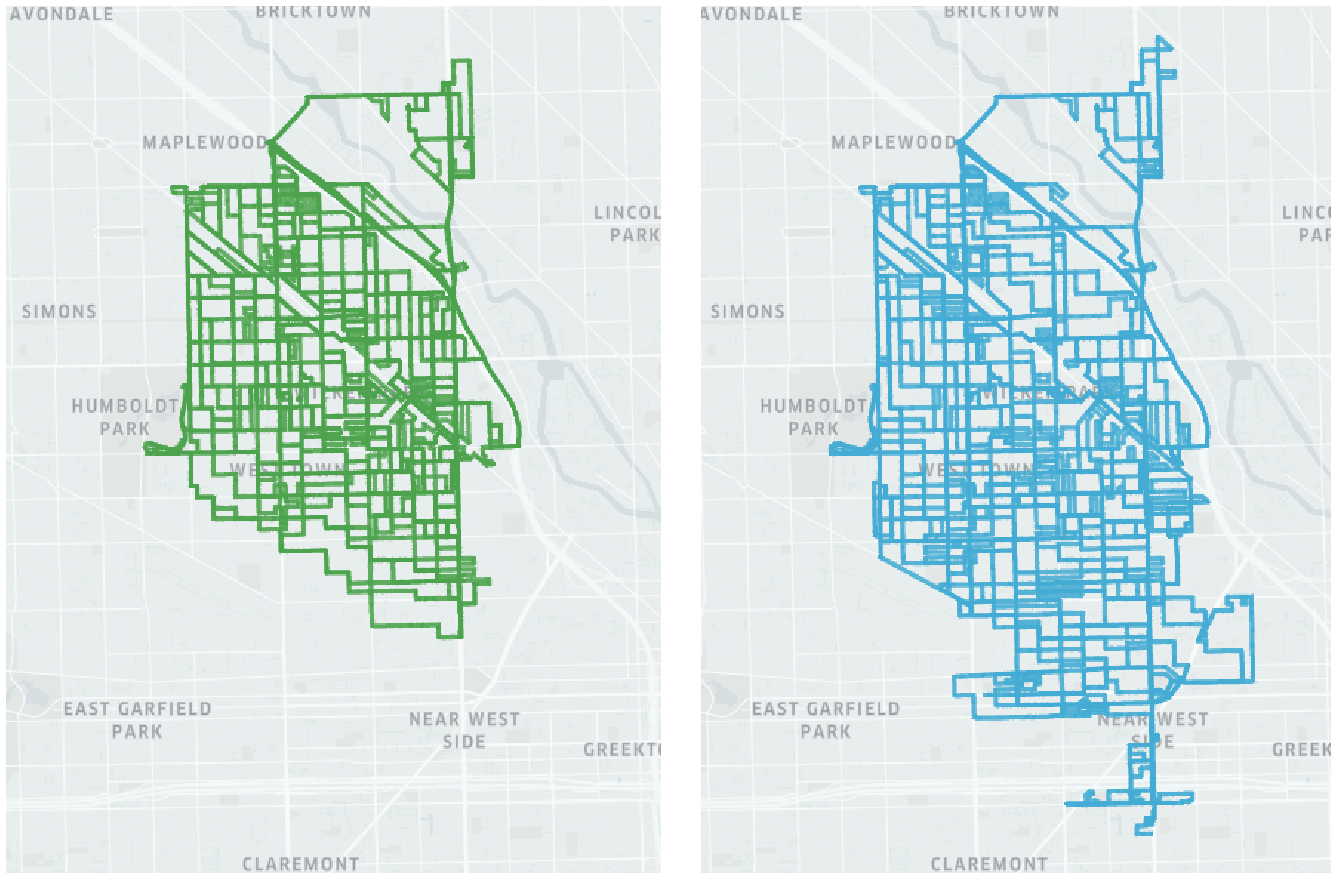
\includegraphics[width=6\textwidth]{figs/il_rl_all.png}
  \else
    \begin{tabular}{ll}
      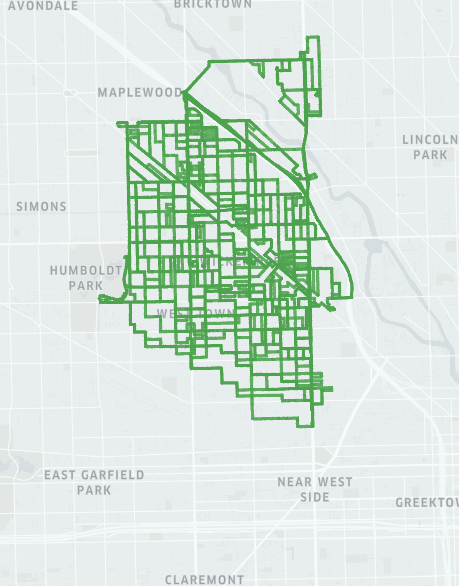
\includegraphics[height=9.1cm,trim={0.2cm 0 0.4cm 0},clip]{figs/il_rl_rl.png} &
      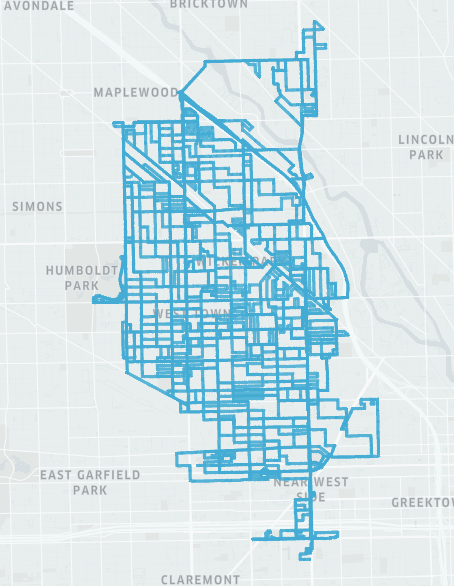
\includegraphics[height=9.1cm,trim={0.2cm 0 0.8cm 0},clip]{figs/il_rl_il.png} \\
    \end{tabular}
  \fi
  % \vspace{-0.15in}
  \caption{Bird's eye view of a partially complete traversal
  of MARVIN trained with RL (left) and MARVIN trained with IL
  (right). Both are relatively thorough while expanding to new
  regions, but the model trained using imitation learning is
  able to cover the regions in a more efficient manner.}
  \label{fig:il_rl}
  \end{center}
\end{figure*}